
%%% Local Variables:
%%% mode: latex
%%% TeX-master: t
%%% End:

\chapter{PARD原型系统实现与验证}
\label{chap:impl}

%FPGA原型设计目标
上一章已经讨论过如何在X86平台上实现PARD,本章讨论如何在gem5全系统模拟器上将PARD机制
实现其中。验证功能可行性,


\section{基础系统选择}

实现PARD原型系统的第一个工作是选择一个合适的基础系统,
PARD对基础系统有以下需求:

\begin{enumerate}
  \item 能够在FPGA环境下综合;
  \item 独立系统,不依靠任何辅助设施即可运行;
  \item 丰富的I/O设备支持,支持Xilinx VC709开发板所提供的外设,如以太网和PCI-Express;
  \item 能够运行Linux操作系统;
  \item 频率/性能足够运行常见Benchmark应用,如SpecCPU、PARSEC等);
  \item 可以运行典型的数据中心应用,如memcached、httpd等;
  \item 具备完整的软件开发环境;
\end{enumerate}

虽然在开源领域有大量可用的处理器软核,如Oracle OpenSPARC T1\cite{sparct1}、
RISC-V\cite{riscv}、OpenRISC\cite{or1k}、LEON3\cite{leon3}等,
但这些软核并不能满足PARD原型系统的需求。
其中OpenSPARC T1和RISC-V目前的FPGA实现并不是一个独立系统,
需要额外的处理器(如MicroBlaze或ARM)作代理以实现访存与I/O操作;
OpenRISC 1200的软件开发环境支持并不完整;
LEON3是目前开源的处理器软核中最为合适的选择,但其对linux内核的支持并不好,
目前只能运行早期的内核版本,同时软件环境也比较老旧,运行数据中心应用存在一定的困难。
一些FPGA厂商也提供了可配置的处理器核,
如Xilinx的MicroBlaze\cite{microblaze}和ARM\cite{zynq},以及Altera的NIOS II\cite{niosii}。

本文最终选择了Xilinx的MicroBlaze作为基础系统,
其处理器采用32位小端RISC架构,实现了单发射5级流水,
支持MMU及虚拟内存,使用AXI4作为外部总线接口\cite{microblaze-ref}。
该处理器软核在Virtex-7型号的FPGA上频率最高能够达到246MHz,
性能是354DMIPs(1.44DMIPs/MHz)\cite{microblaze},能够满足PARD原型系统的需求。

\begin{figure}[tb]
  \centering
  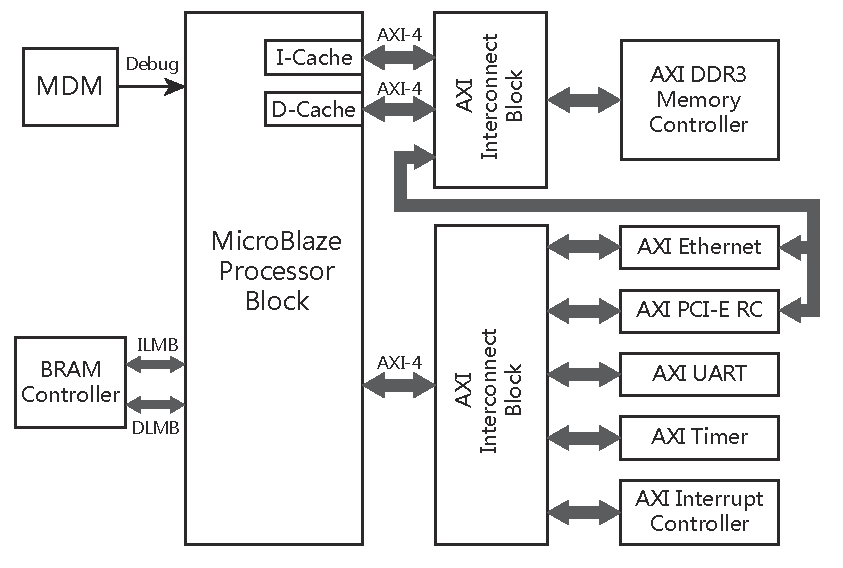
\includegraphics[width=0.6\textwidth]{impl/microblaze-base-arch}
  \caption{MicroBlaze基础架构}
  \label{fig:microblaze-base-arch}
\end{figure}


基于MicroBlaze的一个典型系统架构如图\ref{fig:microblaze-base-arch}所示,
MicroBlaze系统的固件代码保存在Block Memory中,
通过LMB(Local Memory Bus)总线连接到处理器核;
缓存子系统采用哈佛结构,具有分离的指令与数据缓存,它们通过AXI4总线连接到内存控制器;
I/O子系统同样使用AXI4总线互连,其中包括基本的外设,如中断控制器、串口、时钟等,
也支持一些复杂的I/O设备,如以太网\cite{axi-ethernet-subsystem}、
PCI-E\cite{axi-pcie-bridge}等。
MicroBlaze同时还提供了硬件调试接口,可以通过JTAG对其进行调试。

目前Xilinx提供的MicroBlaze软核并不支持多处理器架构,
在硬件实现上没有提供处理器间同步、通信机制,
之前一些工作\cite{microblaze-mp-rsp08,microblaze-mp-xapp}尝试为其增加多处理器支持,
但这些工作只是实现也最底层的处理器间同步、通信机制,
没有可用的操作系统层次上的多核支持。
受到该因素的影响,本文所设计的PARD原型系统只实现了``伪多核''的系统,
即系统中存在多个处理器核,但每个一逻辑域都被限制为只能使用一个处理器核。
未来MicroBlaze的多核软硬件支持完善后,可以很容易的将PARD原型系统的这一限制解除,
实现真正的多核系统。


\section{PARD原型系统}

PARD原型系统架构如图\ref{fig:pard-arch-impl}所示,
该系统由处理器子系统、I/O子系统、PRM SoC三部分组成。
其中处理器子系统包含四个处理器核心、共享缓存和内存控制器;
I/O子系统中包含四个串口控制器、两个以太网控制器和一个PCI Express根逻辑(RootComplex),
系统中所有的数据通路使用AXI4总线连接;
PRM同样是基于MicroBlaze的SoC系统,对外提供串口与SFP以太网接口,
同时通过内部串口与I/O子系统相连,用于接收I/O子系统的串口输出,
使用I2C总线作为控制平面网络的数据链路层,连接到系统中的四个控制平面:
处理器核控制平面CoreCP、共享缓存控制平面CacheCP、内存控制器控制平面MemCP和
I/O子系统控制平面I/OCP。

\begin{figure}[tb]
  \centering
  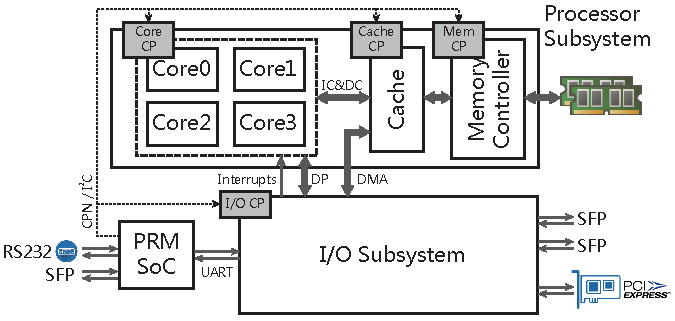
\includegraphics[width=0.8\textwidth]{impl/pard-arch-impl}
  \caption{PARD原型系统架构}
  \label{fig:pard-arch-impl}
\end{figure}

% 如何增加标签寄存器
处理器核心使用MicroBlaze软核及其它附属模块组成,
其内部结构如图\ref{fig:pard-core-impl}所示,
其中包含MicroBlaze软核、中断控制器和时钟模块,
该模块从外部输入时钟、复位和中断信号,
通过三个AXI4接口(IC指令缓存端口、DC数据缓存端口和DP外设端口)与外部交换数据。
AXI4总线协议中使用独立的通道实现读写请求、数据与响应,
其中读写请求中包含用户自定义信号,本文使用该信号在系统中传播应用标签。
由于MicroBlaze并没有开放源代码,处理器核的请求标记工作需要在核外进行:
首先在在核外增加了一个标签寄存器,CoreCP连接到该寄存器,并可以对其内容进行修改;
在IC/DC/DP三个端口外分别增加三个标签模块,
用于将标签寄存器的值附加到AXI4总线AR/AW两个通道的USER信号中,完成请求标记。

% 增加共享缓存模块:支持16路、实现标签传播、实现划分
Xilinx为AXI4总线提供了一个缓存功能的IP核SystemCache\cite{pg118-system-cache},
其默认配置最多只能够支持4路组关联,这对于四核的PARD原型系统来说,
不足以验证缓存容量划分的功能,本文通过修改IP核实现,将其扩展到16路组关联;
按照第\ref{chap:labeladdrspace:}节所述的方式,为该模块增加了标签传播功能;
同时修改其默认LRU替换策略,使其支持按路划分功能,
并通过CacheCP对共享缓存的行为进行控制(参见第\ref{chap:impl:cache}节)。
% 实现的多核
该Cache模块提供MicroBlaze专用接口连接四个处理器核,
同时还提供了通用AXI Master接口连接I/O子系统的DMA通道。
内存控制器与I/O子系统的控制平面提供了地址映射功能,实现四个处理器核的资源划分,
第\ref{chap:impl:memcp}节和第\ref{chap:impl:iocp}节将讨论两个控制平面的实现,
并对第\ref{chap:labeladdrspace}章所提出的全硬件支持的虚拟化和
第\ref{chap:hwresman}章所提出的资源管理功能进行评估。

% 原型的照片
本文使用Xilinx Virtex-7 FPGA(型号xc7vx690tffg1761-2)
在VC709平台上实现了上述PARD原型系统,如图\ref{fig:pard-fpga-board}所示。
该原型系统对外呈现三类接口:一个RS232串口,与PRM的串口相连;
三个SFP接口,其中两个连接到I/O子系统,另外一个与PRM的以太网接口相连;
一个PCI-E Gen3 x4接口,连接到I/O子系统,可以连接兼容的PCI-E设备,
在本例中在该接口连接了一块Intel PCI-E以太网卡(芯片型号82575)。

\begin{figure}[tb]
\begin{minipage}{0.48\textwidth}
  \centering
  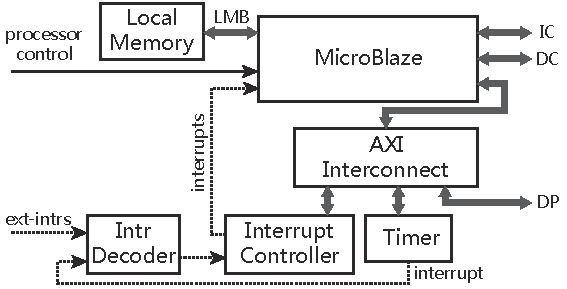
\includegraphics[width=\textwidth]{impl/pard-core-impl}
  \caption{PARD处理器核内部结构}
  \label{fig:pard-core-impl}
\end{minipage}\hfill
\begin{minipage}{0.48\textwidth}
  \centering
  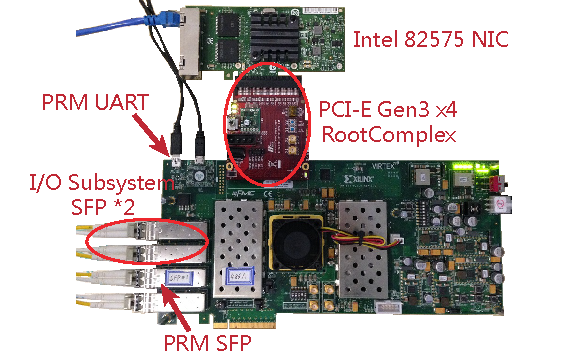
\includegraphics[width=\textwidth]{impl/pard-fpga-board}
  \caption{PARD架构FPGA原型系统}
  \label{fig:pard-fpga-board}
\end{minipage}
\end{figure}

% 资源占用与FPGA布线结果
该原型系统在FPGA上的布局布线结果如图\ref{fig:pard-fpga-routed}所示。

\begin{figure}[tb]
  \centering
  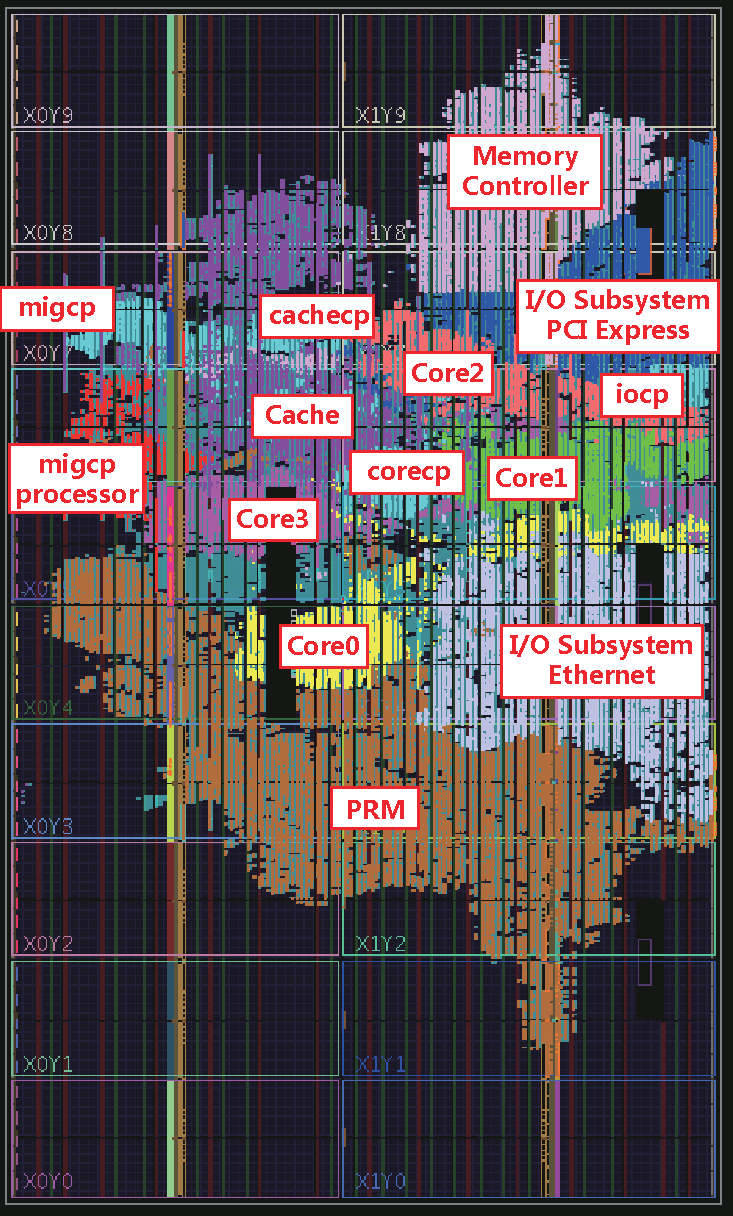
\includegraphics[width=0.8\textwidth]{impl/pard-fpga-routed}
  \caption{PARD原型系统布局布线结果}
  \label{fig:pard-fpga-routed}
\end{figure}



\section{PRM与控制平面网络设计}

为何选择I2C,有何替代

如何改造I2C成为双向网络

连接多个控制平台

触发表中断传播机制


\section{系统设计与关键技术}

\subsection{标签集成}

\subsection{通用控制平面设计}

\subsubsection*{表设计}
\subsubsection*{状态表更新逻辑}
\subsubsection*{触发表逻辑}

\subsection{通用数据平面设计}

\subsection{系统集成}

\subsubsection*{系统集成:处理器核}

\subsubsection*{系统集成:共享末级缓存}

\subsubsection*{系统集成:内存控制器}

\subsubsection*{系统集成:I/O子系统}


\subsection{小结}
包含踩过的坑,如基础系统选择,最初的OpenSPARC方案+寄存器修改 => MicroBlaze外包一层
FPGA实现中遇到的问题


\section{软件栈设计}



\section{性能评估}

\subsection{区分化服务}

\subsection{性能隔离}

\subsection{策略生效时间}

并讨论如何实现ms级控制

\subsection{实际应用测试}

\subsection{开销}


\section{小结}


\if 0	% 模拟器移动到第4、5章相应的章节

\section{模拟器实现}
\subsection{基本配置}

\subsection{模拟器设计目标}

与网络/SDN对比的功能表格,列出实现目标

列出模拟器局限

\subsection{系统设计与关键技术}

\subsubsection{实现全硬件虚拟化}

标签机制 + core/LLC/mc/io
ptable + MultiOS

\subsubsection{实现资源预留}

stable统计 + LLC partition

\subsubsection{实现QoS}

ttable + scheduling + feedback

\subsubsection{管理}

PRM + Program/Trigger

\subsubsection{小结}

总结已实现的功能,并对未来可能扩展的功能进行展望

\subsection{小结}

\fi

